\documentclass{beamer}
\usepackage[english]{babel} 
\usepackage[T1]{fontenc}
\usepackage[ansinew]{inputenc}
\usepackage{lmodern} 
\usepackage{graphicx} 
\usepackage{amsmath}
\usepackage{amsthm}
\usepackage{amsfonts}
\usepackage{float}
\usepackage{amssymb}
\usepackage{graphicx}
\usetheme{Warsaw}

 \newtheorem{Prop}{Proposition}
 \newtheorem{Lm}{Lemma}
 \newtheorem{Th}{Theorem}
 \newtheorem{Def}{Definition}
 \newtheorem{ex}{Example}
 \newtheorem{cor}{Corollary}
 \newtheorem{recap}{Recap}

\DeclareMathOperator{\e}{e}
\newcommand{\esp}[1]{\mathbb{E}\!\left[#1\right]}
\newcommand{\cov}[2]{\text{cov}\!\left(#1,#2\right)}
\newcommand{\var}[1]{\text{Var}\!\left(#1\right)}
\newcommand{\abs}[1]{\left\lvert#1\right\rvert}

\AtBeginSubsection[]
{
\begin{frame}
\frametitle{Plan}
\tableofcontents[currentsubsection]
\end{frame}}
\AtBeginSection[]
{
\begin{frame}
\frametitle{Plan}
\tableofcontents[currentsection, hideallsubsections]
\end{frame}}

\title{The Weighted Majority Algorithm}   
\author{Fabrice Zapfack 
\and Hugo Marival} 
\date{\today} 


\begin{document}
	\begin{frame}[label=titre]
		\titlepage
	\end{frame}
	
	\section{Introduction}
		\subsection{Halving Algorithm}
			\begin{frame}{Halving Algorithm}

				  
				\begin{itemize}
				\item At each step predict the majority vote
				\item Keep only the functions that are consistent
				\end{itemize}
				\begin{Th}
					Let $m$ be the number of mistakes when we apply Halving on $\mathcal{S}$ with the pool $\mathcal{A}$.
					\[m \leq log_2(|A|)\]
				\end{Th}
				\textsc{Attention} - Works only in the realisable case. 
			\end{frame}

		\subsection*{Winnow Algorithm}

	\section{The Weighted Majority Algorithm}
	
\begin{frame}{Framework for WMA}

\textsc{WMA} - Given a pool of algorithms $\mathcal{A}$ where one of them performs well, we will create a compound algorithm based on a weighted voting of the algorithms of $\mathcal{A}$. \newline\newline
\textsc{Different frameworks}  
\begin{itemize}
\item \textbf{WM} - Binary WM predictions, binary pool predictions, deterministic WM and pool algorithms
\item \textbf{WMG} - Binary WM predictions, continuous (in [0,1]) pool predictions, deterministic WM and pool algorithms
\item \textbf{WMC} - Continuous (in [0,1]) WM and pool predictions, deterministic WM and pool algorithms
\item \textbf{WMR} - Continuous (in [0,1]) WM and pool predictions, probabilistic WM and pool algorithms
\end{itemize}

\end{frame}

		\subsection{Classic version - Binary predictions, finite cardinal}
			\subsubsection*{Presentation}
\begin{frame}{Bound on the number of mistakes}

\textsc{Notations} 
\begin{itemize}
\item $\mathcal{S}$ : sequence of instances and binary labels
\item $w_{init}$ : initial total weight of the algorithms in the pool
\item $w_{fin}$ : final total weight of the algorithms in the pool
\item $q_0$ : total weight of the algorithms that predict 0
\item $q_1$ : total weight of the algorithms that predict 1
\item $\beta$ : weight multiplication factor in case of a mistake ($0\leq\beta<1$) 
\end{itemize}

\begin{Th}
Let $m$ be the number of mistakes when we apply WMA on $\mathcal{S}$ with the pool $\mathcal{A}$.
\[m \leq \frac{\mathrm{log}(w_{init}/w_{fin})}{\mathrm{log(2/(1+\beta))}}\]
\end{Th}

\end{frame}
			
			\subsubsection*{Proof}
			
\begin{frame}
\textsc{Proof sketch}  
\begin{itemize}
\item Step 1 - Prove that if in a trial WM makes a mistake, the sum of weights before the trial is greater than $u=\frac{1+\beta}{2}$ times the sum of weights after
\item Step 2 - Recursively, we get that $w_{init}u^m \geq w_{fin}$
\item Step 3 - Take the log of the above inequality to conclude \newline
\end{itemize}

\textsc{Proof of step 1} - Let us suppose wlog that the learner predicted 0 which was the wrong binary label in this trial.
\begin{itemize}
\item Total weight before : $q_0 + q_1$. Since 0 was predicted, $q_0 \geq q_1$
\item Total weight after : $\beta q_0 + q_1 \leq \beta q_0 + q_1 + \frac{1-\beta}{2}(q_0 + q_1) \leq \frac{1+\beta}{2}(q_0 + q_1)$
\end{itemize}
\end{frame}

		\subsection{Modified version}

\begin{frame}{WML - Adaptive version}

\textsc{What motivates this modified version (WML)?}  \newline
\begin{itemize}
\item First version :  selects a group of "good" algorithms and makes other weights shrink
\item Not very good for adaptation : if throughout the trials another group becomes better it will not be seen because of its small weight
\item Idea : Do not allow an algorithm's weight to be lower that $\frac{\gamma}{\lvert\mathcal{A}\rvert}$ times the total weight of $\mathcal{A}$
\end{itemize}
\end{frame}

\begin{frame}{WML - Bounds}

\begin{Lm}
Let $m_0$ be the minimum number of mistakes made on the sequence $\mathcal{S}$ by any algorithm of the pool $\mathcal{A}$ of $n$ algorithms. If the initial weight of each algorithm is at least $\frac{\beta\gamma}{n}$ times the total initial weight, then WML applied to $\mathcal{A}$ makes at most
\[\frac{\mathrm{log}(n/\beta\gamma)+m_0\mathrm{log}(1/\beta)}{\mathrm{log}(1/u)}\]
mistakes, with $u = \frac{1+\beta}{2} + (1 - \beta)\gamma$. The final weight of each algorithm is at least $\frac{\beta\gamma}{n}$ times the total final weight
\end{Lm}

\end{frame}
		
		\subsection{Generalized version - WMG and WMC}
			\subsubsection*{Presentation}
\begin{frame}

\textsc{Assumptions for WMG and WMC} 
\begin{itemize}
\item Predictions of algorithms in the pool in [0,1] for both
\item WMG predictions are binary
\item WMC predictions are in [0,1]
\item Labels are binary for WMG
\item Labels are in [0,1] for WMC \newline
\end{itemize}

\textsc{Update step} 
\begin{itemize}
\item Updates at every trial for WMC
\item Updates either at every trial or only when a mistake occurs
\end{itemize}

\end{frame}	

\begin{frame}

\textsc{Notations}
\begin{itemize}
\item \textit{Update-trial j} : j-th trial  in which an update occurs, $j = 1..t$, $\lvert\mathcal{A}\rvert = n$
\item $x_i^{(j)}$ : prediction of the i-th algorithm in update-trial j
\item $\lambda^{(j)}$ : prediction of the master (compound) algorithm in update-trial j
\item $\rho^{(j)}$ : label of update-trial j
\item $w_1^{(j)}, ..., w_n^{(j)}$ : weights at the beginning of update-trial j
\item $s^{(j)} = \sum_{i=1}^{n}w_i^{(j)}, \gamma^{(j)} = \frac{\sum_{i=1}^{n}w_i^{(j)}x_i^{(j)}}{s^{(j)}}$\newline
\end{itemize}
\textsc{Predictions}
\begin{itemize}
\item WMC : $\lambda^{(j)} = \gamma^{(j)}$
\item WMG : $\lambda^{(j)} = 1$ if $\gamma^{(j)} \geq \frac{1}{2}$ and $\lambda^{(j)} = 0$ if $\gamma^{(j)} < \frac{1}{2}$
\end{itemize}

\end{frame}		

			\subsubsection*{WMG - Bound and proof}

\begin{frame}{Bound for WMG}

\begin{Def}[Update step for WMG and WMC]
$w_i^{(j+1)} = F w_i^{(j)}$ where $F = F(\beta,x_i^{(j)},\rho^{(j)})$ satisfies : 
\[\beta^{\lvert x_i^{(j)} - \rho^{(j)} \rvert} \leq F \leq 1-(1-\beta)\lvert x_i^{(j)} - \rho^{(j)} \rvert\] 
\end{Def}

\begin{Th}[Bound for WMG]
Let $m$ be the number of mistakes when running WMG on $\mathcal{S}$ with $0 \leq \beta <1$.
\[m \leq \frac{\mathrm{log}(w_{init}/w_{fin})}{\mathrm{log(2/(1+\beta))}}\]
\end{Th}

\end{frame}
		
\begin{frame}{Bound for WMG - Proof}

Let us start by proving that we can always find an update factor F :
\begin{Lm}
For $\beta \geq 0$ and $0 \leq r \leq 1$ : $\beta^r\leq 1 + r(\beta - 1)$
\end{Lm}
\textsc{Proof} - Convexity inequality on $r \mapsto \beta^r$\newline
In the following lemma, we will assume that $w_i^{(1)}>0$, $\rho^{(j)}\leq 1$ and $0\leq x_i^{(j)}\leq 1$ for $i=1..n, j=1..t$. 

\end{frame}

\begin{frame}

\begin{Lm}[5.2]
Let us also assume that for $i=1..n, j=1..t, w_i^{(j+1)}\leq w_i^{(j)}(1-(1-\beta)\lvert x_i^{(j)}-\rho^{(j)}\rvert)$. If $\beta=0$ and $\lvert \gamma^{(j)}-\rho^{(j)}\rvert=1$ for some $j$, then $w_{fin} = 0$. Otherwise,
\[\mathrm{log}(\frac{w_{fin}}{w_{init}})\leq\sum_{j=1}^{t}\mathrm{log}(1-(1-\beta)\lvert \gamma^{(j)}-\rho^{(j)}\rvert)\]
\end{Lm}
\textsc{Proof}.\newline
First case - If $\beta=0$ and $\lvert \gamma^{(j)}-\rho^{(j)}\rvert=1$ for some $j$. Then 
\begin{align*}
\lvert \frac{\sum_i w_i^{(j)}x_i^{(j)}}{\sum_i w_i^{(j)}} - \frac{\sum_i w_i^{(j)}\rho^{(j)}}{\sum_i w_i^{(j)}} \rvert &= 1\\
\Rightarrow\lvert \frac{\sum_i w_i^{(j)}(x_i^{(j)} - \rho^{(j)})}{\sum_i w_i^{(j)}} \rvert &= 1\\
\end{align*}

\end{frame}

\begin{frame}{Proof of Lemma 5.2 (..page 2..)}
\[\Rightarrow\frac{\sum_i w_i^{(j)}\lvert x_i^{(j)} - \rho^{(j)}\rvert}{\sum_i w_i^{(j)}} \geq 1\]
Since $x_i^{(j)}, \rho^{(j)}\in [0,1]$, $\lvert x_i^{(j)} - \rho^{(j)} \rvert \leq 1$, so $\frac{\sum_i w_i^{(j)}\lvert x_i^{(j)} - \rho^{(j)}\rvert}{\sum_i w_i^{(j)}}$ can only be greater than 1 if $\lvert x_i^{(j)} - \rho^{(j)} \rvert = 1$ for $i=1..n$, so we have to use the update factor ($\beta = 0$) and $w_i^{(j+1)} = 0$ for $i = 1..n$ so $w_{fin} = 0$. \newline \newline
Second case - Using the convexity inequality from the proof of a previous lemma :
\[s^{(j+1)}\leq\sum_{i=1}^{n} w_i^{(j)}(1-(1-\beta)\lvert x_i^{(j)}-\rho^{(j)}\rvert) = s^{(j)} - (1 - \beta)\sum_{i=1}^{n} w_i^{(j)}\lvert x_i^{(j)}-\rho^{(j)}\rvert\]

\end{frame}

\begin{frame}{Proof of Lemma 5.2 (..end)}

Using the triangular inequality:
\begin{align*}
s^{(j)} - (1 - \beta)\sum_{i=1}^{n} w_i^{(j)}\lvert x_i^{(j)}-\rho^{(j)}\rvert &\leq s^{(j)} - (1 - \beta)\lvert\sum_{i=1}^{n} w_i^{(j)}(x_i^{(j)}-\rho^{(j)})\rvert\\
																																						&= s^{(j)} - (1 - \beta)\lvert\sum_{i=1}^{n} \gamma^{(j)}s^{(j)}-\rho^{(j)}s^{(j)}\rvert\\
																																						&= s^{(j)}(1 - (1 - \beta)\lvert\gamma^{(j)} -\rho^{(j)}\rvert)
\end{align*}
Recursively, we get :
\[s^{(t+1)} \leq s^{(1)}\prod_{j=1}^{t}(1 - (1 - \beta)\lvert\gamma^{(j)} -\rho^{(j)}\rvert)\]
\end{frame}

\begin{frame}{Proof of the WMG bound}

\textsc{Proof of the WMG bound}.
First case - $\beta = 0 \Rightarrow w_{fin} = 0$ so the bound becomes ...
Second case - Let $m^{(j)} = 1$ if WMG makes a mistake in update-trial j, 0 otherwise. $m=\sum_{j=1}^{t} m^{(j)}$.\newline
Since $\mathrm{log}(1-(1-\beta)\lvert\gamma^{(j)} - \rho^{(j)}\rvert)\leq 0$,
\[\sum_{j=1}^{t}\mathrm{log}(1-(1-\beta)\lvert\gamma^{(j)} - \rho^{(j)}\rvert)\leq \sum_{j\text{ s.t. }m^{(j)}=1}\mathrm{log}(1-(1-\beta)\lvert\gamma^{(j)} - \rho^{(j)}\rvert)\]
\begin{itemize}
\item If $\gamma^{(j)}<\frac{1}{2}$, $m^{(j)}=1\Rightarrow\rho^{(j)}=1\Rightarrow\lvert\gamma^{(j)} - \rho^{(j)}\rvert\geq\frac{1}{2}$
\item If $\gamma^{(j)}\geq\frac{1}{2}$, $m^{(j)}=1\Rightarrow\rho^{(j)}=0\Rightarrow\lvert\gamma^{(j)} - \rho^{(j)}\rvert\geq\frac{1}{2}$
\end{itemize}

\end{frame}

\begin{frame}{Proof of the WMG bound (..end)}

So, 
\[\sum_{j\text{ s.t. }m^{(j)}=1}\mathrm{log}(1-(1-\beta)\lvert\gamma^{(j)} - \rho^{(j)}\rvert)\leq m\mathrm{log}(1-\frac{1}{2}(1-\beta)) = m\mathrm{log}(\frac{1}{2}+\frac{1}{2}\beta)\]
We can use Lemma 5.2 and get :
\[\mathrm{log}(\frac{w_{fin}}{w_{init}})\leq m\mathrm{log}(\frac{1+\beta}{2})\]

\end{frame}

			\subsubsection*{WMC - Bound and proof}

\begin{frame}{Bound for WMC}

\begin{Def}[Loss m  for WMC]
For continuous predictions, the loss is defined by :
\[m = \sum_{j=1}^{t}\lvert\lambda^{(j)} - \rho^{(j)}\rvert\]
\end{Def}

\begin{Th}
Let $\mathcal{S}$ be any sequence of instances and labels, with labels in [0,1]. Let m be the total  loss for the WMC.
\[m\leq\frac{\mathrm{log}(w_{init}/w_{fin})}{1-\beta}\]
\end{Th}

\end{frame}

\begin{frame}

\begin{Lm}[5.3]
If the conditions of Lemma 5.2 are satisfied, then 
\[\sum_{j=1}^{t}\abs{\gamma^{(j)} - \rho^{(j)}} \leq \frac{\mathrm{log}(w_{init}/w_{fin})}{1 - \beta}\]
\end{Lm}
\textsc{Proof}
\[\mathrm{log}(1 - (1 - \beta)\abs{\gamma^{(j)} - \rho^{(j)}}) \leq - (1 - \beta)\abs{\gamma^{(j)} - \rho^{(j)}}\]
We then use Lemma 5.2 to get the bound.

\end{frame}

		
		\subsection{Randomized version}
			\subsubsection*{Presentation}

\begin{frame}

\textsc{Assumptions}
\begin{itemize}
\item Predictions of pool members are in [0,1]
\item Prediction of WMR is binary but probabilistic
\item Labels associated with instances are binary\newline
\end{itemize}

\textsc{Prediction of WMR}
\begin{itemize}
\item WMR predicts 1 with probability $\gamma^{(j)}$
\item If pool members' predictions are binary, $\gamma^{(j)} = \frac{q_1}{q_0+q_1}$.\newline
\end{itemize}

\textsc{Update criterion}
\begin{itemize}
\item Update in every trial\newline
\end{itemize}

\textsc{Update step}
\begin{itemize}
\item Same update step as WMG and WMC.
\end{itemize}

\end{frame}

\begin{frame}{Weak independence}

In WMR, $x_i^{(j)}$ and $\rho^{(j)}$ are random variables. In order to count the mistakes made by WMR, we will use the following assumption :\newline
\textsc{Weak independence condition}
\[\esp{\lambda^{(j)}|(x^{(1)}, \rho^{(1)}), .., (x^{(j)}, \rho^{(j)})} = \gamma^{(j)}\text{ for }j=1..t\]
\textsc{Remark}
If $x_i^{(j)}$ and $\rho^{(j)}$ are chosen deterministically then all of the weights and $\gamma^{(j)}$ are also deterministic and the construction of the algorithm gives us that 
\[\esp{\lambda^{(j)}|(x^{(1)}, \rho^{(1)}), .., (x^{(j)}, \rho^{(j)})} = \esp{\lambda^{(j)}} = \gamma^{(j)}\]

\end{frame}

\begin{frame}{Strong independence}

To give a bound on the concentration of the total number of mistakes around it's mean, we will use the following assumption:\newline
\textsc{Strong independence condition}
\[\esp{\lambda^{(j)}|(x^{(1)}, \rho^{(1)}), .., (x^{(t)}, \rho^{(t)}), \lambda^{(1)}, .., \lambda^{(j-1)}} = \gamma^{(j)}\]
\textsc{Remark}\newline
Strong independence $\Rightarrow$ weak independence.

\end{frame}

\begin{frame}{Bound on the expected number of mistakes}

\begin{Th}
Let $\mathcal{S}$ be a sequence of instances with binary labels. Let $m$ be the number of mistakes made by WMR on $\mathcal{S}$ when applied to a pool of probabilistic prediction algorithms. If the weak independence condition holds,
\[\esp{m}\leq\frac{\esp{\mathrm{log}(w_{init}/w_{fin})}}{1 - \beta}\]
\end{Th}
\textsc{Proof}\newline
Weak indep. condition : $\esp{\abs{\lambda^{(j)} - \rho^{(j)}}|(x^{(1)}, \rho^{(1)}), .., (x^{(j)}, \rho^{(j)})} = \abs{\gamma^{(j)} - \rho^{(j)}}$.\newline
So $\esp{\abs{\lambda^{(j)} - \rho^{(j)}}} = \esp{\abs{\gamma^{(j)} - \rho^{(j)}}}$.

\end{frame}

\begin{frame}

\begin{align*}
\esp{m} &= \esp{\sum_{j=1}^{t}\abs{\lambda^{(j)} - \rho^{(j)}}} \\
				&= \esp{\sum_{j=1}^{t}\abs{\gamma^{(j)} - \rho^{(j)}}}
\end{align*}
Then we use Lemma 5.3

\end{frame}

\begin{frame}{Recap of the algorithms and their bounds}

\begin{recap}[WMA \& WMG]
\[\frac{\mathrm{log}(n) + m\mathrm{log}(1/\beta)}{\mathrm{log}(2/(1+\beta))}\]
\end{recap}


\begin{recap}[WMC \& WMR]
\[\frac{\mathrm{log}(n) + m\mathrm{log}(1/\beta)}{1 - \beta}\]
\end{recap}


\end{frame}


			\subsubsection*{Proof}
			
	\section{Improvements}
		\subsection{Exponentially Weighted Aggregation (EWA)}
			\begin{frame}{EWA}

				  
				\begin{itemize}
				\item fix $p_1 = \pi$ an arbitrary probability distribution on $\mathbb{R}^M$ 
				\item $\hat{y}_t=\int f_\theta (x_t) p_t({\rm d})\theta$ and once $y_t$ is revealed,
$$ p_{t+1}({\rm d}\theta) = \frac{
\exp\left(-\eta \ell(y_t,f_\theta (x_t)) \right) p_{t}({\rm d}\theta)
}{
\int_{\mathbb{R}^M} \exp\left(-\eta \ell(y_t,f_\alpha (x_t)) \right) p_{t}({\rm d}\alpha)
}. $$
				\end{itemize}
				\begin{Th}
					Taking $\eta=2\sqrt{\frac{2\log(M)}{T C^2}}$ leads to a regret in
$$
\mathcal{R}_T(\{f_1,\dots,f_M\}) \leq C \sqrt{\frac{T \log(M)}{2}}.
$$
				\end{Th}
				\textsc{Attention} - Applicable to L-type, C-type, MS-type aggregation
			\end{frame}


\section{Applications}
		\subsection{Applicable case}

\begin{frame}
	\frametitle{Randomly generated samples }
	\begin{figure}
		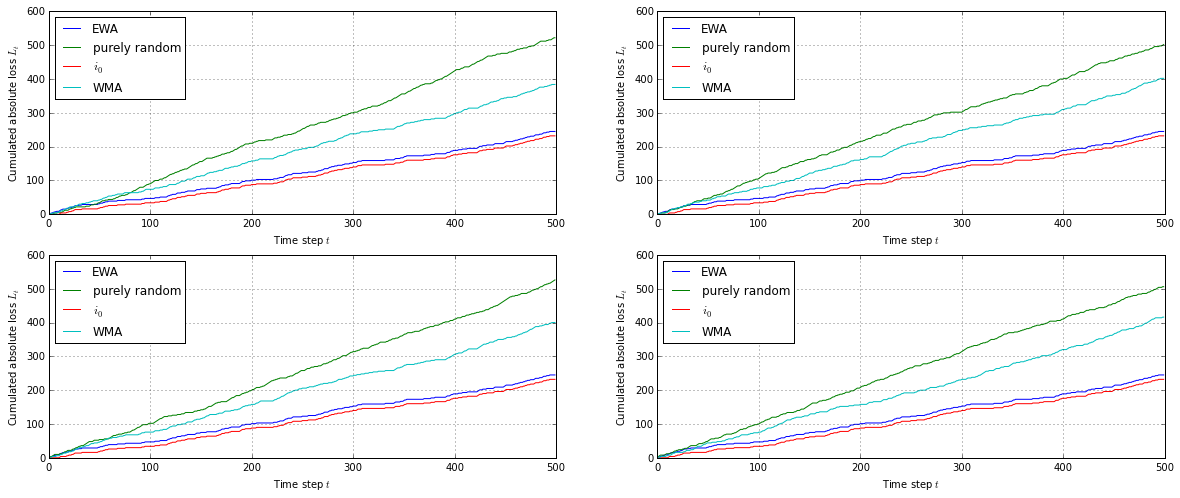
\includegraphics[scale=0.25]{download.png}
	\end{figure}
\end{frame}
\begin{frame}
	\frametitle{Randomly generated samples }
	\textsc{WMA1} - Initials weights are normally distributed
	\begin{figure}
		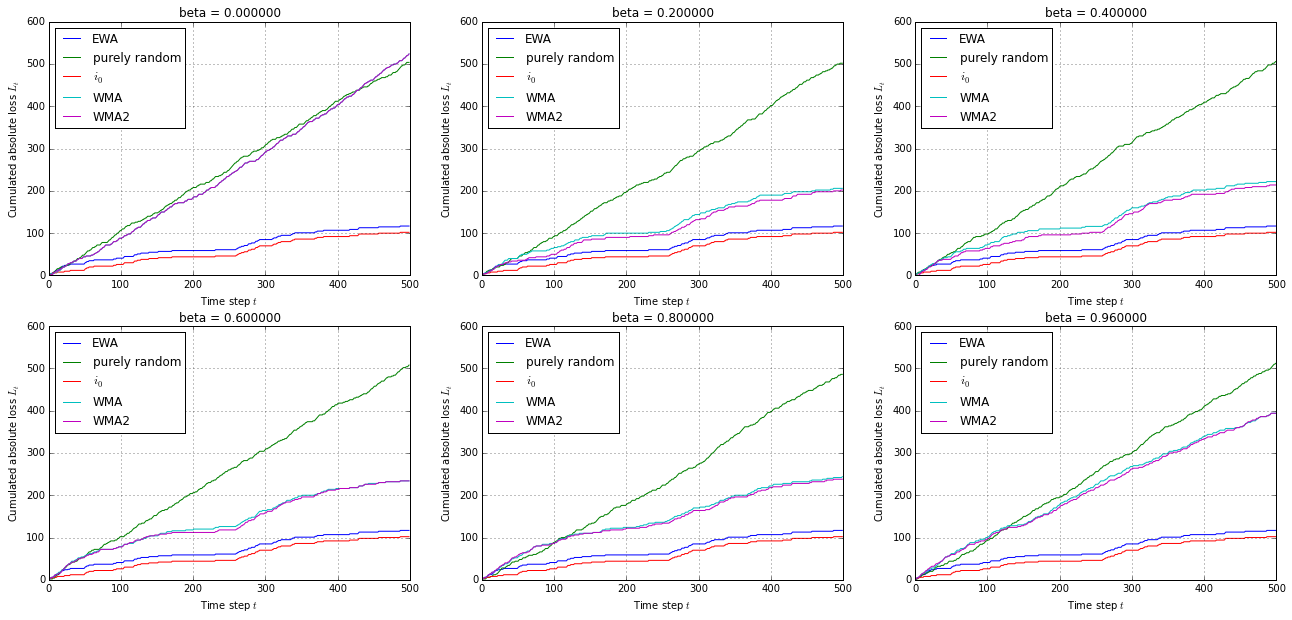
\includegraphics[scale=0.25]{download2.png}
	\end{figure}
\end{frame}

		\subsection{Non-applicable case}

\begin{frame}
	\frametitle{Exercise 6 (TD): Observations are randomly given }
	\begin{figure}
		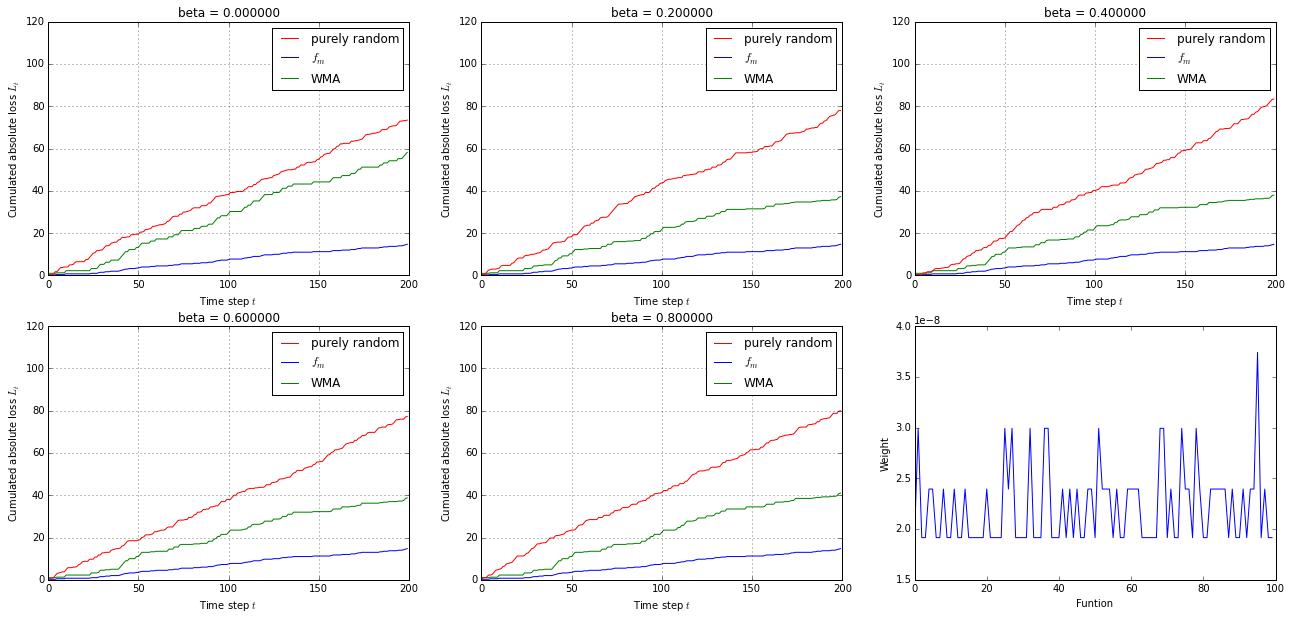
\includegraphics[scale=0.25]{exo6.png}
	\end{figure}
\end{frame}
\begin{frame}
	\frametitle{Exercise 6 (TD): Observations are given in the order of the paper }
	\begin{figure}
		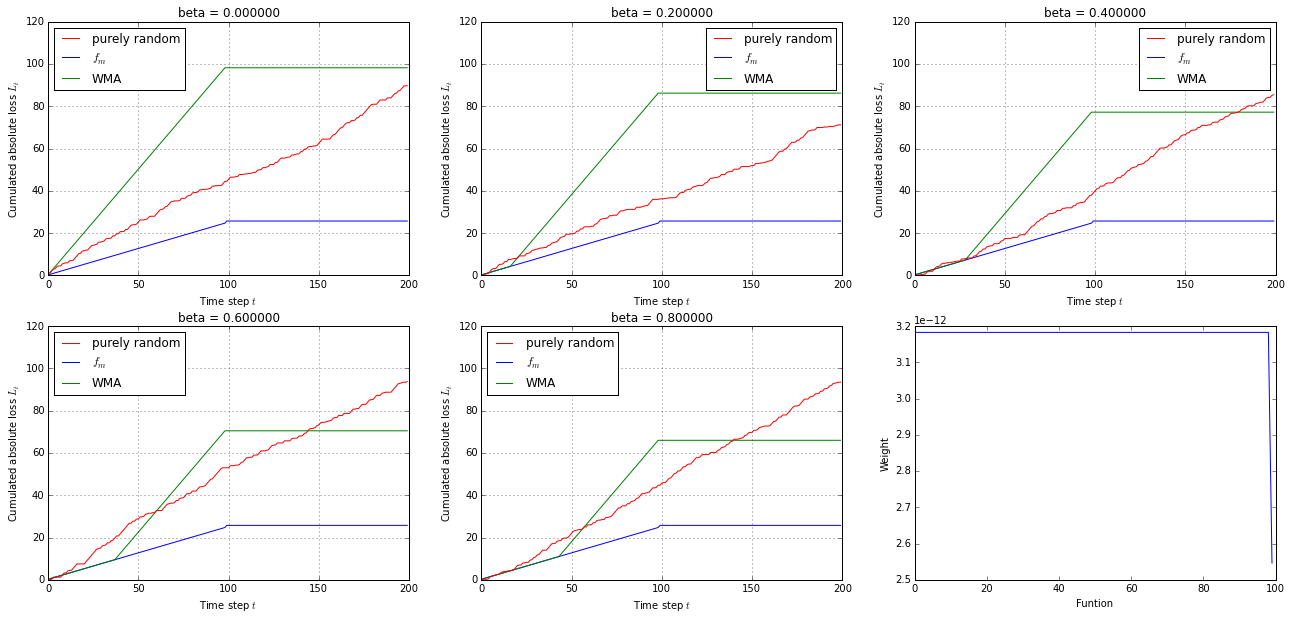
\includegraphics[scale=0.25]{exo6_ordered.png}
	\end{figure}
\end{frame}

		%\subsection{Non-applicable case}
\end{document}
